Phase correlation is a technique used in digital signal processing to register two signals, images or 3D volumes with translation differences. It is robust to noise and view-point changes. Techniques in phase correlation can also be used to find additional parameters (such as rotation, scale and sheer). Fourier methods such as phase correlation can therefore be used to compute camera pose without the need for non-linear methods such as ICP, which cannot recover scaling parameters and has several other inadequacies (see section \ref{ICPSection}). \\ 

In this section we describe 2D phase correlation. The 2D version of phase correlation is important to discuss as techniques are applied directly to the 3D version (described in chapter \ref{FVRSectionA}) which is important for this research. \\

Phase correlation is part of an area of research and applications named Digital Signal Processing (DSP). DSP is the scientific area concerned with the acquisition, filtering, processing and understanding of digital signals using computer technology. Digital signals are simply an array of numbers, digital images are 2D signals and digital volumes are 3D signals. One of the fundamental ideas behind this research area is that digital signals can be processed using a set of common techniques regardless of where or how they were generated. There are two fundamental techniques used in digital signal processing. One is the use of correlation and convolution, the other is the use of alternative representations ie the Fourier transform \cite{Smith97Scientist}. \\

Convolution is the process by which one signal is used to filter another whilst correlation is used to measure the similarity between one signal and another at different phases. The Fourier transform is used to transform signals (in the time domain) into the frequency domain. The frequency domain represents the original signal using a set of sine and cosine waves at different frequencies. The time domain is the name given to the original domain of the signal. This transform is performed by correlating the signal with sine and cosine waves at varying frequencies. A transform called the inverse Fourier transform can be used to transform a signal from the frequency domain back to the time domain. \\

The inputs and outputs of the Fourier transform are digital signals made up of complex numbers. Most of the time, the input signal is not complex (as in the case of a photographed scene). In this case imaginary value scalars of zero are augmented to the signal to make it complex. The frequency domain can be visualized easily using the polar representation of these complex numbered signals. The polar representation represents the signal using the magnitude and phase of sine waves at different frequencies and directions (in the case of 2D). This can be visualized in figure \ref{fig:PCSecA}, here the magnitude represents the height of the sine waves, the phase represents the translation from the origin in which these waves occur and the 2D position within the image represents the direction the waves travel in 2D. The most useful aspect of the Fourier transform is that when signals are represented in the frequency domain, their point-wise multiplication is equivalent to convolution in the time domain. This is important because convolution is a computationally intensive process, especially in image processing where there is a lot of data to process. \\

\begin{figure*}[t!] 
        \centering
        \begin{subfigure}[b]{4.5cm}
                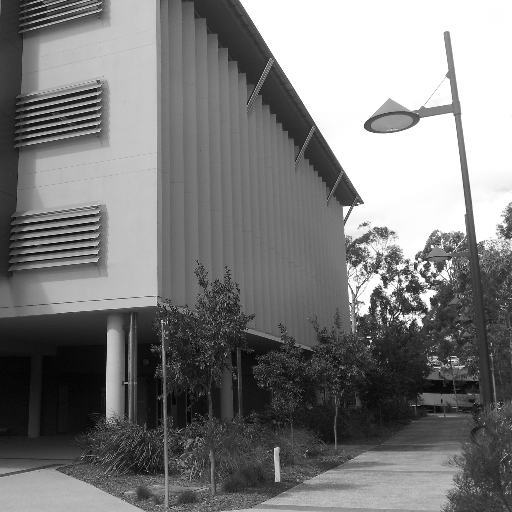
\includegraphics[width=4.2cm]{images/pc/original}
                \caption{original}
                \label{fig:PCSecOrig1}
        \end{subfigure}%
        \begin{subfigure}[b]{4.5cm}
                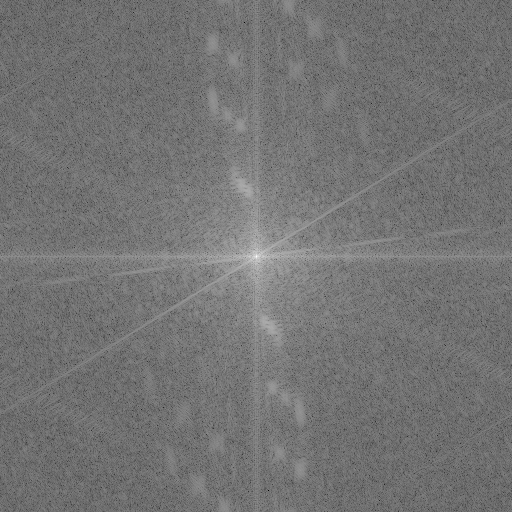
\includegraphics[width=4.2cm]{images/pc/magnitude}
                \caption{magnitude}
                \label{fig:PCSecMag}
        \end{subfigure}%
                \begin{subfigure}[b]{4.5cm}
                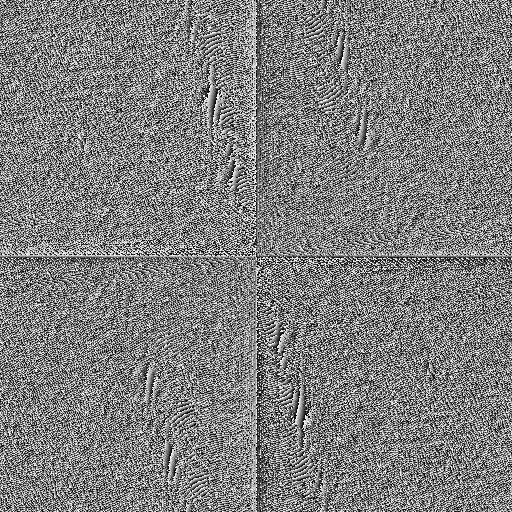
\includegraphics[width=4.2cm]{images/pc/phase}
                \caption{phase}
                \label{fig:PCSecPhase}
        \end{subfigure}%        
       \caption{The polar representation of the Discrete Fourier transform on an input image.}\label{fig:PCSecA}
\end{figure*}

Phase correlation is the process of using the frequency domain representation to perform image registration using correlation. In image processing, this allows us to find the translation parameters between two images (it does not work if rotation or scaling are introduced) efficiently. This can be performed by flipping one image before transforming both into the frequency domain. Since point-wise multiplication in the frequency domain causes convolution in the time domain, flipping one image causes correlation in the frequency domain which is what is required. Once this correlation is performed, the inverse Fourier transform is performed, the output image contains a peak which is used to compute the translation difference between the two images. This can be visualized in figure \ref{fig:PCSecCC}. Here, the original image is translated from figure \ref{fig:PCSecORY} to figure \ref{fig:PCSectrans} and the two are phase correlated producing the peak in figure \ref{fig:PCSecCCPC} which represents the translation between the two. \\


\begin{figure*}[t!] 
        \centering
        \begin{subfigure}[b]{4.5cm}
                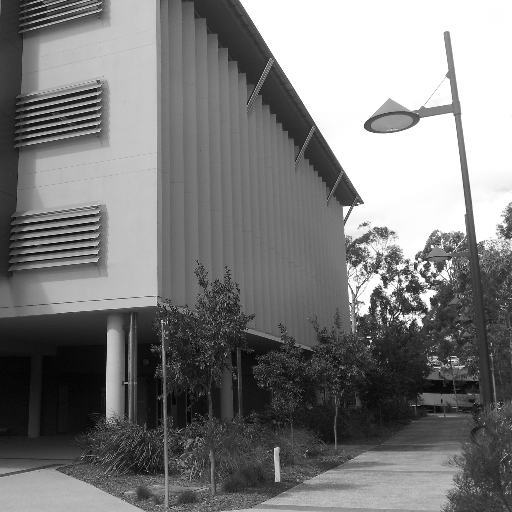
\includegraphics[width=4.2cm]{images/pc/original}
                \caption{original}
                \label{fig:PCSecORY}
        \end{subfigure}%
        \begin{subfigure}[b]{4.5cm}
                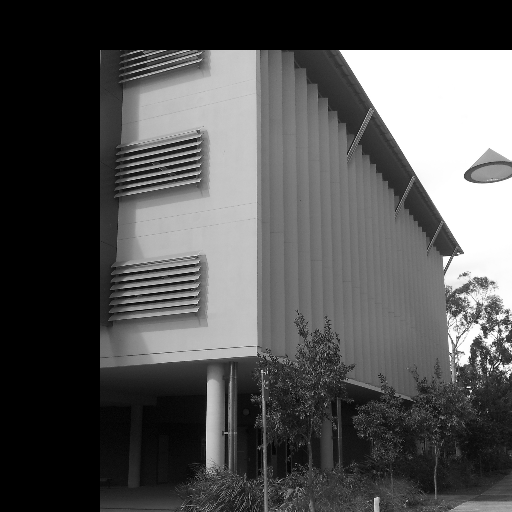
\includegraphics[width=4.2cm]{images/pc/translated}
                \caption{(a) translated}
                \label{fig:PCSectrans}
        \end{subfigure}%
                \begin{subfigure}[b]{4.5cm}
                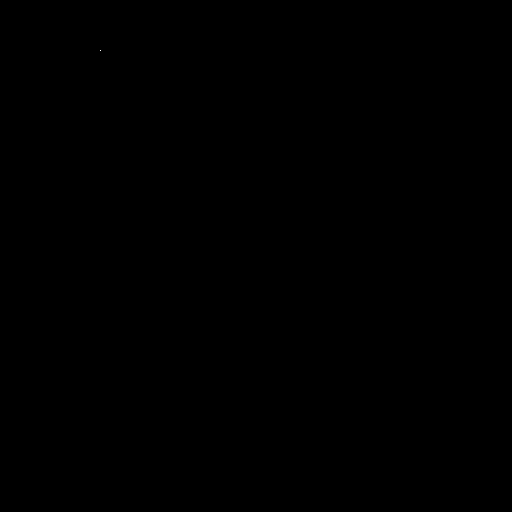
\includegraphics[width=4.2cm]{images/pc/phasecorrelation1}
                \caption{correlation}
                \label{fig:PCSecCCPC}
        \end{subfigure}%        
       \caption{Phase correlation used to align two images seperated by a translation.}\label{fig:PCSecCC}
\end{figure*}

The other parameters we wish to estimate for registration are the scale and rotation parameters, however another type of transform is introduced first. This image transform is called the log-polar transform. This transform re-arranges the pixels from euclidean 2D space $[x,y]$ to the polar space $[log(sqrt(x^2+y^2)),atan(y/x)]$ where rotation about the centre is turned into y-axis translation and scaling about the centre is turned into x-axis translation. This representation changes any rotation and scaling performed on the image into translation. Translation parameters can be easily found using phase correlation. This process can be visualized with the help of figure \ref{fig:PCSecB}. The problem is, the rotation and scaling has to be about the centre of the image, which is an issue if the images contain a translation effects. Luckily, in the magnitude of the polar representation of the frequency domain the effects of translation are not present. On top of this, any rotation or scaling (whether translation is present or not) occurs about the centre of the image. \\

\begin{figure*}[t!] 
        \centering
        \begin{subfigure}[b]{3.4cm}
                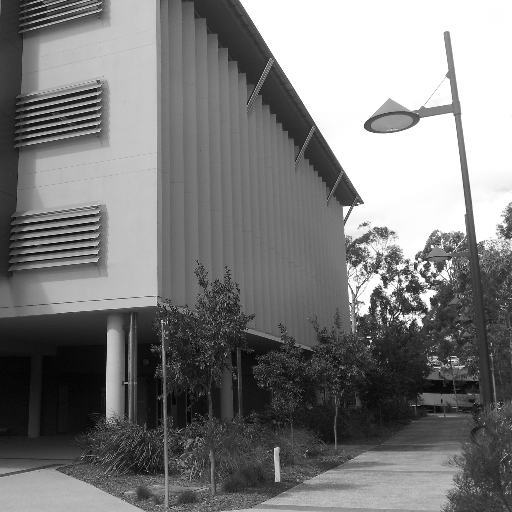
\includegraphics[width=3.2cm]{images/pc/original}
                \caption{original}
                \label{fig:PCSecOrig2}
        \end{subfigure}%
        \begin{subfigure}[b]{3.4cm}
                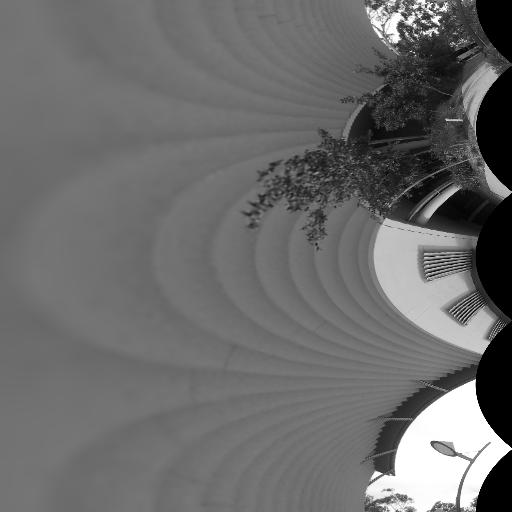
\includegraphics[width=3.2cm]{images/pc/logpolar}
                \caption{log-polar(a)}
                \label{fig:PCSecLP}
        \end{subfigure}%
         \begin{subfigure}[b]{3.4cm}
                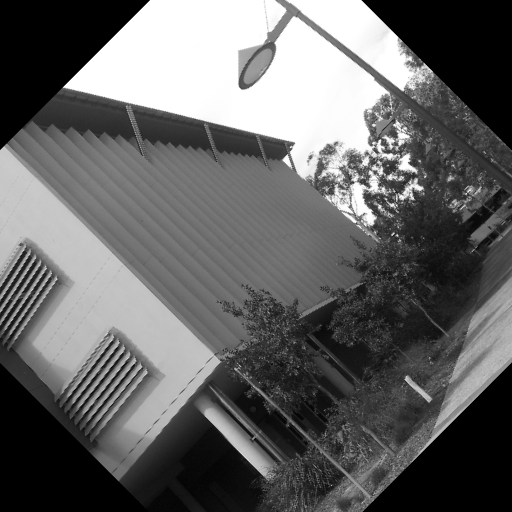
\includegraphics[width=3.2cm]{images/pc/rotation}
                \caption{rotated (-45${}^{\circ}$)}
                \label{fig:PCSecRot}
        \end{subfigure}%
        \begin{subfigure}[b]{3.4cm}
                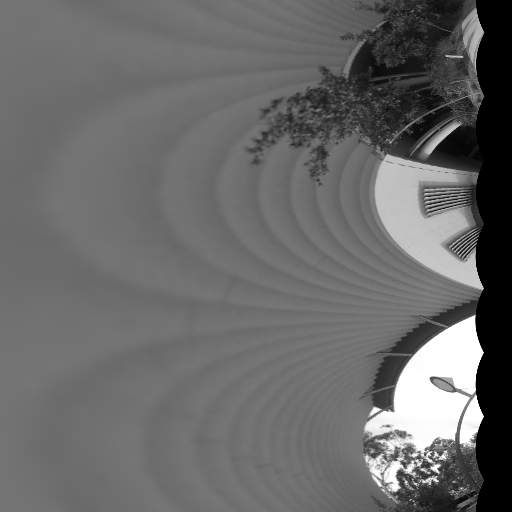
\includegraphics[width=3.2cm]{images/pc/logpolarRotation}
                \caption{log-polar(b)}
                \label{fig:PCSecLPR}
        \end{subfigure}
         \begin{subfigure}[b]{3.4cm}
                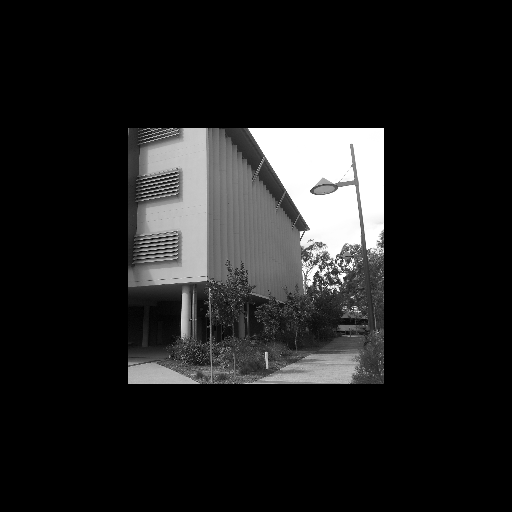
\includegraphics[width=3.2cm]{images/pc/scaled}
                \caption{scaled $\times$0.5}
                \label{fig:PCSecOrig2}
        \end{subfigure}%
        \begin{subfigure}[b]{3.4cm}
                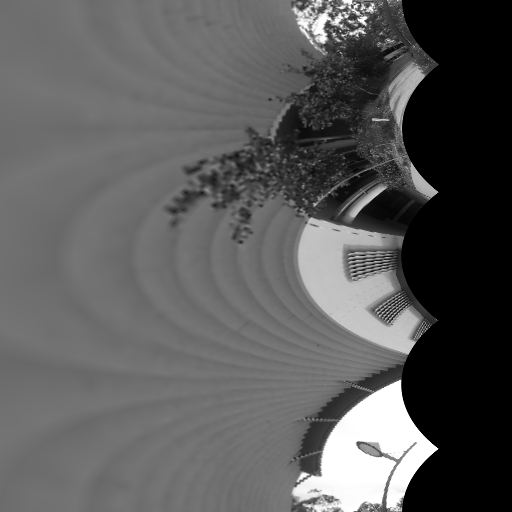
\includegraphics[width=3.2cm]{images/pc/logpolarScale}
                \caption{log-polar(c)}
                \label{fig:PCSecLP}
        \end{subfigure}%
                \begin{subfigure}[b]{3.4cm}
                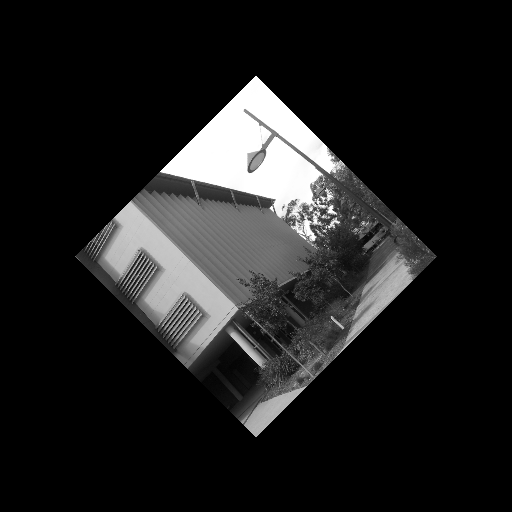
\includegraphics[width=3.2cm]{images/pc/rotationscale}
                \caption{rotated \& scaled}
                \label{fig:PCSecRot}
        \end{subfigure}%
        \begin{subfigure}[b]{3.4cm}
                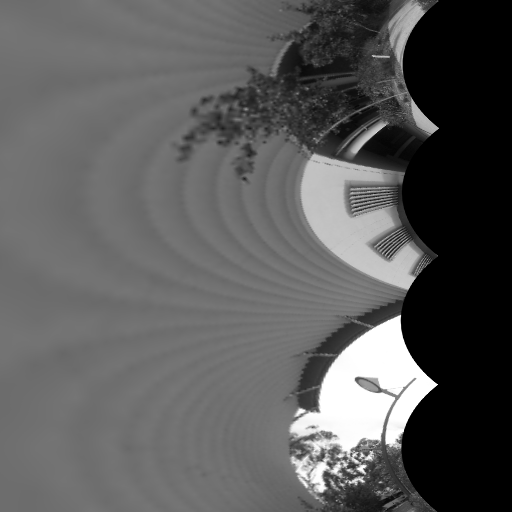
\includegraphics[width=3.2cm]{images/pc/logpolarRotationScale}
                \caption{log-polar(d)}
                \label{fig:PCSecLPR}
        \end{subfigure}%        
       \caption{The effects of the log polar transform.}\label{fig:PCSecB}
\end{figure*}

This allows the phase correlation method to recover the translation, scaling and rotational information between two images. First, the magnitude of the polar representation of both the images is computed. Then both magnitudes are log-polar transformed and phase correlated. This finds the scaling and rotational parameters. Both of the original images have their rotation and scaling reversed, then both images are phase correlated to undo the effects of translation, which is the final parameter to compute. In this way, translation, scaling and rotational parameters can be computed directly without the need for feature matching. \\
